\documentclass[a4paper,12pt]{article}
\usepackage[a4paper,top=1.3cm,bottom=2cm,left=1.5cm,right=1.5cm,marginparwidth=0.75cm]{geometry}

% Пакеты
\usepackage{mathtext} 
\usepackage{setspace}
\usepackage{tabularx}
\usepackage{cmap}
\usepackage{longtable}
\usepackage{icomma}
\usepackage{euscript}
\usepackage{float}
\usepackage{cutwin}
\usepackage{mathrsfs}
\usepackage{adjustbox}
\usepackage{dashbox}
\usepackage[normalem]{ulem}
\usepackage[T2A]{fontenc}			
\usepackage[utf8]{inputenc}                 %!  закрепляет кодировку utf8
\usepackage[english,russian]{babel}         %!  подключает русский и английский
%математические шрифты:
\usepackage{amsmath,amsfonts,amssymb,amsthm,mathrsfs,mathtools} 
\usepackage[colorlinks, linkcolor = purple]{hyperref}      %!  оглавление для панели навигации по PDF-документу + гиперссылки
\usepackage{xcolor}                         %!  добавляет цвета
\usepackage{enumitem}                       %!  задание макета перечня.
\usepackage{xpatch}                         %?  работа с renewcommand и макросами              
\usepackage{cancel}                         %   зачёкивания текста (!!!) для slash-нотации использовать \usepackage{slashed}!!
\usepackage{upgreek}                        %   заглавные греческие буквы
\usepackage{lipsum}                         %?  для вставки кучи текста при форматировании
\usepackage[version=4]{mhchem}              %   химические формулы
\usepackage{multirow}                       %   объединение строк в матрицах
\usepackage{stackengine}                    %   stack символов
\usepackage{tikz}                           %!  рисунки
\usetikzlibrary{positioning}                %?  библиотека для тикза 
\usepackage{titletoc}                       %!  форматирование содержания и заголовков
\usepackage{titlesec}                       %!  форматирование содержания и заголовков
\usepackage{wrapfig}                        %   обтекание таблиц и рисунков
\usepackage{chngcntr}                       %!  для setcounter
\usepackage{fancyhdr}                       %!  для колонтитулов
\usepackage{makecell}                       %?  матрицы с разными выравниваниями и т.п
\usepackage{indentfirst}                    %   добавить indent перед первым 
\usepackage{tocloft}                        %?  изменение названий глав и разделов                       
\usepackage{soul}                           %   типографические примочки, типо зачёркивания и подчёркивания
\usepackage[stable]{footmisc}               %?  продвинутые сноски
\usepackage{subfig}                         %   несколько картинок рядом
%  задаёт поля страниц

% pgf plots
% \usepackage{pgfplots}
% \pgfplotsset{compat=1.17}

\mathtoolsset{showonlyrefs=true}

%Обозначения теорем и т.п
\theoremstyle{definition}
\newtheorem*{definition}{Определение}
\newtheorem{statement}{Предложение}[section]
\newtheorem{lemma}{Лемма}[section]
\newtheorem{theorem}{Теорема}[section]
\newtheorem*{theoremn}{Теорема}
\newtheorem*{corollary}{Следствие}
\newtheorem*{example}{Пример}
\newtheorem*{note}{Замечание}
\newtheorem*{problem}{Задача}

%Шарабара для содержания и внешнего вида нумерации
\counterwithout{footnote}{section}\DeclareRobustCommand{\divby}{%
	\mathrel{\text{\vbox{\baselineskip.65ex\lineskiplimit0pt\hbox{.}\hbox{.}\hbox{.}}}}%
}



%Толерантный квадратик чтд
%\makeatletter \renewenvironment{proof}[1][\proofname]{\par\pushQED{\qed}\normalfont\topsep6\p@\@plus6\p@\relax\trivlist\item[\hskip\labelsep\bfseries#1\@addpunct{.}]\ignorespaces}{\popQED\endtrivlist\@endpefalse} \makeatother
%\renewcommand\qedsymbol{$\squareulblack$}
%\newcommand{\usubseteq}{\mathbin{\rotatebox[origin=c]{90}{$\subset$}}}
%\DeclareFontEncoding{LS2}{}{\noaccents@}
%\DeclareFontSubstitution{LS2}{stix}{m}{n}
%\DeclareSymbolFont{arrows3}{LS2}{stixtt}{m}{n}
%\DeclareMathSymbol{\squareulblack}{\mathord}{arrows3}{"88}

%Разные операторы и символы
\newcommand{\dotpr}[2]{\bra{#1}\ket{#2}}
\let\AA\relax
%\let\oldvarphi\phi %оно делает так, что \phi становится правильным фи
%\let\phi\varphi
%\let\varphi\oldvarphi
\let\emptyset\varnothing
\DeclareMathOperator*{\esssup}{ess sup}
\DeclareMathOperator*{\ord}{ord}
\DeclareMathOperator*{\supp}{supp}
\DeclareMathOperator*{\pr}{pr}
\DeclareMathOperator*{\Ker}{Ker}
\DeclareMathOperator*{\Vol}{Vol}
\DeclareMathOperator*{\rg}{rk}
\DeclareMathOperator*{\Ima}{Im}
\DeclareMathOperator*{\Alt}{Alt}
\DeclareMathOperator*{\Sym}{Sym}
\newcommand{\eqdef}{\stackrel{\text{\tiny{def}}}{=}}
\newcommand{\pp}{\partial}
\newcommand{\AA}{\mathcal{A}}
\newcommand{\BB}{\mathcal{B}}
\newcommand{\MM}{\mathbb{M}}
\newcommand{\NN}{\mathbb{N}}
\newcommand{\ZZ}{\mathbb{Z}}
\newcommand{\QQ}{\mathbb{Q}}
\newcommand{\RR}{\mathbb{R}}
\newcommand{\CC}{\mathbb{C}}
\newcommand{\FFF}{\mathbb{F}}
\newcommand{\DD}{\mathcal{D}}
\newcommand{\FF}{\mathcal{F}}
\newcommand{\sS}{\mathcal{S}}
\newcommand*\circled[1]{\tikz[baseline=(char.base)]{
		\node[shape=circle,draw,inner sep=2pt] (char) {#1};}}

\graphicspath{ {./images/2.1.3} }


\title{Определение $C_p$/$C_v$ по скорости звука в газе (2.1.3)}
\author{Павлушкин Вячеслав}
\date{\today}


\begin{document}
	\maketitle
	
	\section{Введение}
	\noindent\textbf{Цель работы:}  
	\begin{enumerate}
		\item измерение частоты колебаний и длины волны при резонансе звуковых колебаний в газе, заполняющем трубу;
		\item определение показателя адиабаты с помощью уравнения состояния идеального газа.
	\end{enumerate}
	
	\textbf{В работе используются:} звуковой генератор ГЗ; электронный осциллограф ЭО; микрофон; телефон; раздвижная труба; теплоизолированная труба, обогреваемая водой из термостата; баллон со сжатым углекислым газом; газгольдер.
	
	\section{Теоретические сведения}
	
	Скорость распространения звуковой волны в газах зависит от показателя адиабаты $\gamma $. На измерении скорости звука основан один из наиболее точных методов определения показателя адиабаты.
	
	Скорость звука в газах определяется формулой:
	
	\begin{equation}
		c=\sqrt{\gamma\frac{RT}{\mu}}.
		\label{velocity}
	\end{equation}
	где $ R $ -- газовая постоянная, $ T $ -- температура газа, а $ \mu $ -- его молярная масса. Преобразуя эту формулу, найдем
	\begin{equation}\label{gamma}
		\boxed{\gamma = \frac{\mu}{RT}c^2}.
	\end{equation}
	
	Таким образом, для определения показателя адиабаты достаточно измерить температуру газа и скорость распространения звука (молярная масса газа предполагается известной).
	
	Звуковая волна, распространяющаяся вдоль трубы, испытывает многократные отражения от торцов. Звуковые колебания в трубе являются наложением всех отраженных волн и очень сложны. Картина упрощается, если длина трубы $ L $ равна целому числу полуволн, то есть когда \[ L=n\lambda/2, \] где $ \lambda $ -- длина волны звука в трубе, а $ n $ -- любое целое число. Если это условие выполнено, то волна, отраженная от торца трубы, вернувшаяся к ее началу и вновь отраженная, совпадает по фазе с падающей. Совпадающие по фазе волны усиливают друг друга. Амплитуда звуковых колебаний при этом резко возрастает -- наступает резонанс.
	
	При звуковых колебаниях слои газа, прилегающие к торцам трубы, не испытывают смещения. Узлы смещения повторяются по всей длине трубы через $ \lambda/2 $. Между узлами находятся максимумы смещения.
	
	Скорость звука c связана с его частотой $ f $ и длиной волны $ \lambda $ соотношением
	
	\begin{equation}\label{lambda_f}
		c=\lambda f.
	\end{equation}
	
	Подбор условий, при которых возникает резонанс, можно производить двояко:
	\begin{enumerate}
		\item При неизменной частоте $ f $ звукового генератора (а следовательно, и неизменной длине звуковой волны $ \lambda $) можно изменять длину трубы $ L $. Для этого применяется раздвижная труба. Длина раздвижной трубы постепенно увеличивается, и наблюдается ряд последовательных резонансов. Возникновение резонанса легко наблюдать на осциллографе по резкому увеличению амплитуды колебаний. Для последовательных резонансов имеем \begin{equation}\label{first}
			L_n=n\frac{\lambda}{2}, \quad L_{n+1}=(n+1)\frac{\lambda}{2}, \quad \dots, \quad L_{n+k} = n\frac{\lambda}{2}+k\frac{\lambda}{2},
		\end{equation} т. е. $ \lambda/2 $ равно угловому коэффициенту графика, изображающего зависимость длины трубы $ L $ от номера резонанса $ k $. Скорость звука находится по формуле \eqref{lambda_f}.
		\item При постоянной длине трубы можно изменять частоту звуковых колебаний. В этом случае следует плавно изменять частоту $ f $ звукового генератора, а следовательно, и длину звуковой волны $ \lambda $. Для последовательных резонансов получим 
		\begin{equation}\label{4}
			L=\frac{\lambda_1}{2}n=\frac{\lambda_2}{2}(n+1)=\dots=\frac{\lambda_{k+1}}{2}(n+k).
		\end{equation}
		
		Из \eqref{lambda_f} и \eqref{4} имеем:
		\[ f_1=\frac{c}{\lambda_1}=\frac{c}{2L}n, \quad f_2=\frac{c}{\lambda_2}=\frac{c}{2L}(n+1)=f_1+\frac{c}{2L},\quad \dots, \]
		\begin{equation}\label{5}
			f_{k+1}=\frac{c}{\lambda_{k+1}}=\frac{c}{2L}(n+k)=f_1+\frac{c}{2L}k.
		\end{equation}
		Скорость звука, деленная на $ 2L $, определяется, таким образом, по угловому коэффициенту графика зависимости частоты от номера резонанса.
	\end{enumerate}
	
	\section{Экспериментальная установка}
	
	Соответственно двум методам измерения скорости звука в работе имеются две установки (рис. \ref{img1} и \ref{img2}). В обеих установках звуковые колебания в трубе возбуждаются телефоном Т и улавливаются микрофоном М. Мембрана телефона приводится в движение переменным током звуковой частоты; в качестве источника переменной ЭДС используется звуковой генератор ГЗ. Возникающий в микрофоне сигнал наблюдается на осциллографе ЭО.
	
	Микрофон и телефон присоединены к установке через тонкие резиновые трубки. Такая связь достаточна для возбуждения и обнаружения звуковых колебаний в трубе и в то же время мало возмущает эти колебания: при расчетах оба торца трубы можно считать неподвижными, а влиянием соединительных отверстий пренебречь.
	
	Первая установка (рис. \ref{img1}) содержит раздвижную трубу с миллиметровой шкалой. Через патрубок (на рисунке не показан) труба может наполняться воздухом или углекислым газом из газгольдера. На этой установке производятся измерения $ \gamma $ для воздуха и для $ CO_2 $. Вторая установка (рис. \ref{img2}) содержит теплоизолированную трубу постоянной длины. Воздух в трубе нагревается водой из термостата. Температура газа принимается равной температуре омывающей трубу воды. На этой установке измеряется зависимость скорости звука от температуры.
	
	\begin{figure}[H]
		\begin{center}
			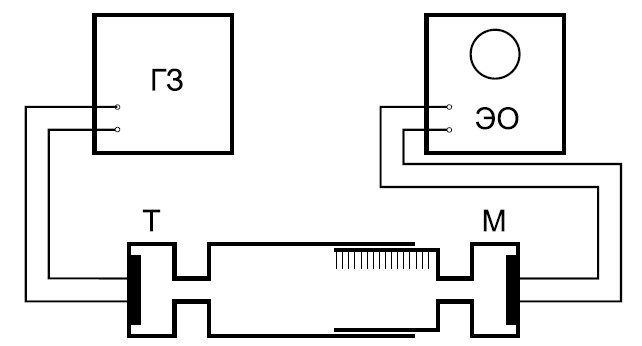
\includegraphics[width=12cm]{ust1.jpg}
		\end{center}
		\caption{\textit{Установка для измерения скорости звука при помощи раздвижной трубы}}
		\label{img1}
	\end{figure}
	
	\begin{figure}[H]
		\begin{center}
			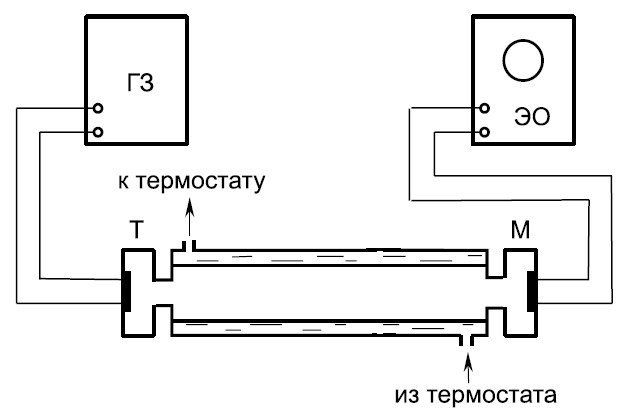
\includegraphics[width=12cm]{ust2.jpg}
		\end{center}
		\caption{\textit{Установка для изучения зависимости скорости звука от температуры}}
		\label{img2}
	\end{figure}
	
	\section{Ход работы}
	
	\subsection{Измерение $ C_p/C_v $ для воздуха при помощи установки с раздвижной трубой}
	
	\label{ident}
	
	Проведём измерение коэффициента $ C_p/C_v $ для воздуха при помощи установки с раздвижной трубой. Для проведения серии измерений фиксируем частоту звукового сигнала и оставляем её неизменной при до окончания снятия показаний. Увеличиваем и уменьшаем длину трубки, чтобы добиться резонанса, возникновение которого устанавливается при помощи осциллографа. При возникновении резонанса фиксируем то расстояние, на которое была выдвинута трубка прибора. Данные измерения проводим для нескольких значений частот. Полученные результаты заносим в таблицу \ref{tab:oxy}.
	
	\begin{table}[H]
		\centering
		\begin{tabular}{|c|c|c|c|c|c|}
			\hline
			$ f $, Гц & \textbf{3643}  &\textbf{3920}  & \textbf{4562}& \textbf{4850}& \textbf{5180} \\ \hline
			$ k $ &  $ \Delta L $, мм & $\Delta L $, мм &$\Delta L $, мм & $\Delta L $, мм &  $\Delta L $, мм \\ \hline
			1&0&0&0&0&0\\ \hline
			2&50&44&38&34&33\\\hline
			3&98&87&75&72&68\\\hline
			4&145&133&113&105&100\\\hline
			5&193&176&151&144&135\\\hline
			6&&222&188&176&167\\\hline
			7&&&227&217&202\\\hline
			
		\end{tabular}
		\caption{Результаты измерений для воздуха}
		\label{tab:oxy}
	\end{table}
	
	Для каждого измерения величины <<выдвига>> трубы $ \sigma_l = 0,5 $ мм. Также для каждого измерения вычислим $ \Delta L = L - l_0 $. Погрешность определения этой величины составит $ \sigma_{\Delta L}=~\sqrt{2}\sigma_l \approx~0,7 $~мм.
	
	По полученным данным построим графики зависимости $ \Delta L(k) $.
	
	\begin{figure}[h!]
		\centering
		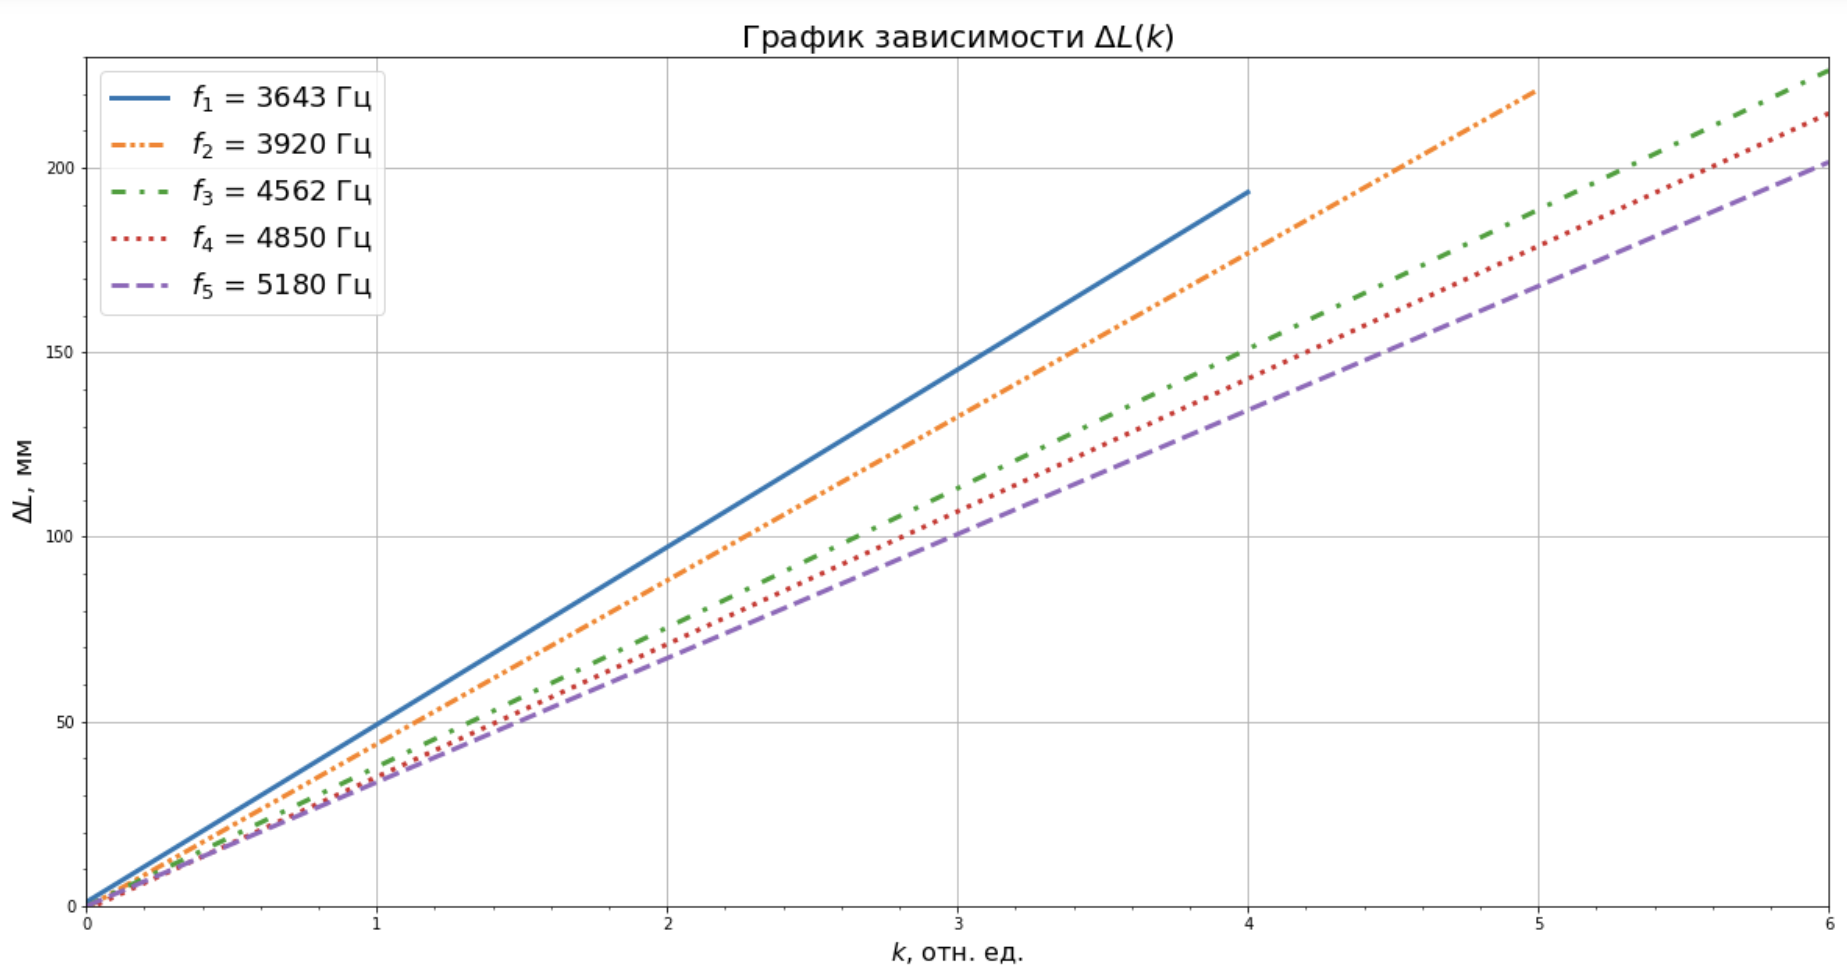
\includegraphics[scale=0.542]{graph1}
		\caption{Зависимость $ \Delta L $ от $ k $ для воздуха}
		\label{graph1}
	\end{figure}
	
	Аппроксимируем полученные зависимости прямыми $ y=ax $ используя метод наименьших квадратов. Коэффициент $ a $ находим согласно следующей формуле:
	
	\begin{equation}\label{mnk:a}
		a=\frac{\left\langle k\Delta L \right\rangle}{\left\langle k^2 \right\rangle}.
	\end{equation}
	

	
	Случайную погрешность определения $ a $ оценим следующим образом:
	
	\begin{equation}\label{mnk:sigma_a}
		\sigma^\text{случ}_a=\sqrt{\frac{1}{N-1}\left(\frac{\left\langle \Delta L^2 \right\rangle}{\left\langle k^2 \right\rangle}-a^2\right)},
	\end{equation}
	где $ N $ -- колличество измерений. Систематическая погрешность определения $ a $ равна $ \sigma_a^\text{сист} = \sigma_{\Delta L} $. Тогда полная погрешность определения коэффициента $ a $ может быть вычислена по следующей формуле:
	
	\begin{equation}\label{mnk:full_sigma}
		\sigma_a=\sqrt{\left(\sigma^\text{случ}_a\right)^2+\left(\sigma^\text{сист}_a\right)^2}.
	\end{equation}
	
	Используя эти формулы вычисляем коэффициенты $ a $ для каждого значения частоты $ f $. результаты вычислений заносим в таблицу \ref{tab:resO2}.
	
	\begin{table}[H]
		\centering
		\begin{tabular}{|c|c|c|c|c|c|c|}
			\hline
			$ f $, Гц & $ a $, мм & $ \sigma_a $, мм & $ \lambda $, мм & $ \sigma_\lambda $, мм & $ c $, м/с & $ \sigma_c $, м/с \\ \hline
			3643 & 48,1 & 0,3 & 96,2 & 0,6 & 350,5 & 2,2 \\ \hline
			3920 & 44,3 & 0,2 & 88,6 & 0,4 & 347,3 & 1,6 \\ \hline
			4562 & 37,8 & 0,1 & 75,6 & 0,2 & 344,9 & 0,9 \\ \hline
			4850 & 36,0 & 0,4 & 71,9 & 0,8 & 348,7 & 3,9 \\ \hline
			5180 & 33,6 & 0,1 & 67,2 & 0,2 & 348,1 & 1,0 \\ \hline
		\end{tabular}
		\caption{Результаты вычислений для воздуха}
		\label{tab:resO2}
	\end{table}
	
	Согласно \eqref{first}, угловой коэффициент наклона прямой $ a $ равен $ \lambda/2 $. По этой формуле вычислим $ \lambda $ и результаты также занесём в таблицу \ref{tab:resO2}.
	
	Согласно \eqref{lambda_f}, скорость звука в воздухе можно вычислить по следующей формуле: 
	\[ c = \lambda f. \]
	
	Погрешность такого вычисления равна \[ \sigma_c=c\sqrt{\varepsilon_f^2+\varepsilon_\lambda^2}. \] При этом в каждом измерении примем $ \sigma_f \approx 1 $ Гц.
	
	Эти результаты также заносим в таблицу \ref{tab:resO2}.
	
	Таким образом, мы получили значение $ c $ для каждого отдельного значения частоты. Усредняя вычисленные значения, в итоге получаем \[\boxed{ c = (347,9 \pm 1,9) \text{ м/с}}\quad (\varepsilon=0,5\%) \]
	
	Также, по формуле \eqref{gamma}, вычислим $ C_p/C_v $:
	
	\[ \frac{C_p}{C_v} = \gamma = \frac{\mu}{RT}c^2. \]
	
	При этом для воздуха $ \displaystyle \mu \approx 0,02898 \text{ } \frac{\text{кг}}{\text{моль}} $. Во время эксперимента температура в лаборатории равнялась $ T = (26,0 \pm 0,1) \text{ } ^\circ C $. Тогда погрешность такого вычисления можно оценить по следующей формуле:
	\[ \sigma_\gamma = \gamma\sqrt{\varepsilon_f^2+\left(2\varepsilon_c\right)^2}.\]
	
	В итоге получаем:
	
	\[ \boxed{\gamma = 1,412 \pm 0,008}\quad (\varepsilon=0,6\%) \]
	
	\subsection{Измерение $ C_p/C_v $ для углекислого газа при помощи установки с раздвижной трубой}
	
	В этой части работы проведём измерения, аналогичные проведённым в п. \ref{ident}, для трубы, заполненной углекислым газом. Заносим результаты измерений зависимости номера резонанса от величины, на которую выдвинута труба, в таблицу \ref{tab:CO2}.

	\begin{table}[!htb]
		
		\begin{minipage}{.5\linewidth}
			\centering
			\begin{tabular}{|c|c|}
				\hline
				$ f $, Гц & \textbf{3727}  \\ \hline
				$ k $ & $  L $, мм   \\ \hline
				0 & 16 \\ \hline
				1 & 87 \\ \hline
				2 & 160 \\ \hline
				3 & 230 \\ \hline
			\end{tabular}
		\end{minipage}%
		\begin{minipage}{.5\linewidth}
			\centering
			\begin{tabular}{|c|c|}
				\hline
				$ f $, Гц & \textbf{4412}  \\ \hline
				$ k $ & $  L $, мм   \\ \hline
				0 & 17 \\ \hline
				1 & 47 \\ \hline
				2 & 77 \\ \hline
				3 & 110 \\ \hline
				4 & 138 \\ \hline
				5 & 169 \\ \hline
				6 & 198 \\ \hline
				7 & 230 \\ \hline
			\end{tabular}
		\end{minipage}
		\caption{Результаты измерений для углекислого газа}
		\label{tab:CO2}
	\end{table}
	
	Строим графики зависимости $ L(k) $. Аппроксимируем зависимости прямыми $ y=ax+b $. Результаты заносим в таблицу \ref{tab:resCO2}. Вычисляем также $ \lambda $ и $ c $ для каждого значения частоты $ f $.
	
	\begin{figure}[h!]
		\centering
		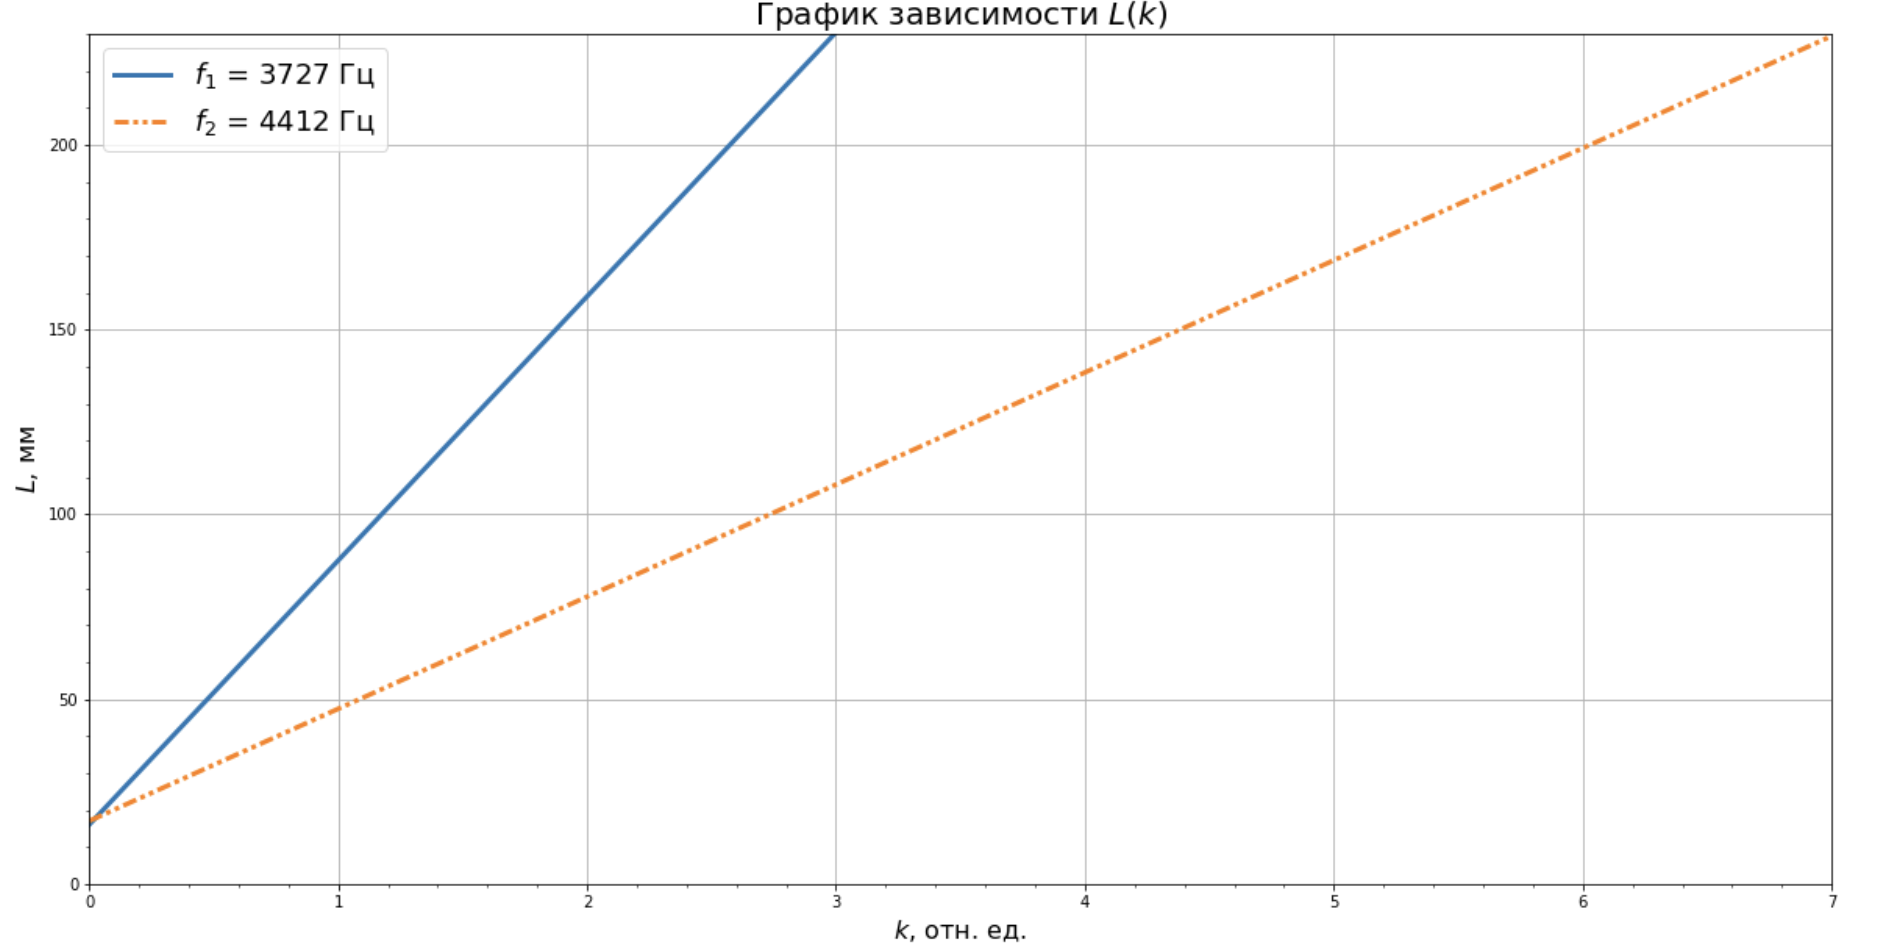
\includegraphics[scale=0.542]{graph3}
		\caption{Зависимость $ L $ от $ k $, для углекислого газа}
		\label{graph2}
	\end{figure}
	
	\begin{table}[H]
		\centering
		\begin{tabular}{|c|c|c|c|c|c|c|}
			\hline
			$ f $, Гц & $ a $, мм & $ \sigma_a $, мм & $ \lambda $, мм & $ \sigma_\lambda $, мм & $ c $, м/с & $ \sigma_c $, м/с \\ \hline
			3727 & 71,5 & 0,4 & 143 & 0,8 & 532,9 & 3,0 \\ \hline
			4412 & 30,4 & 0,2 & 60,7 & 0,8 & 267,9 & 3,5 \\ \hline
		\end{tabular}
		\caption{Результаты вычислений для углекислого газа}
		\label{tab:resCO2}
	\end{table}

	
	Видимо при первом опыте что-то пошло не так, возможно мы неправильно двигали трубку, непонятно, поэтому, получаем:
	
	\[ \boxed{c=(267,9 \pm 3,5)  \text{ м/с}} \quad (\varepsilon=1,3\%)\]
	
	Вычисляя $ C_p/C_v $ аналогично п. \ref{ident}, получаем
	
	\[ \boxed{\gamma = 1,271 \pm 0,016}\quad (\varepsilon=1,4\%) \]
	
	\subsection{Измерение $ C_p/C_v $ для воздуха при различных температурах}
	
	Проведём измерения $ C_p/C_v $ для воздуха при различных температурах. Для этого будем использовать трубу постоянного размера $ L = (700 \pm 1) $ мм. Для фиксированной температуры будем изменять частоту звукового сигнала, тем самым изменяя и длину волны, так, чтобы мы могли наблюдать последовательные резонансы. Для каждого резонанса будем фиксировать частоту, при которой он возник. Полученные измерения занесём в таблицу \ref{tab:constL}.
	
	\begin{table}[H]
		\centering
		\begin{tabular}{|c|c|c|c|c|c|}
			\hline
			$ T $, К & \textbf{294,4} & \textbf{303,6} & \textbf{313,4} & \textbf{323,2}& \textbf{333,2}  \\ \hline
			$k$ &  $ f_k $, Гц & $ f_k $, Гц &  $ f_k $, Гц & $ f_k $, Гц & $ f_k $, Гц \\ \hline
			0 & 262 &266 & 269&273&275  \\ \hline
			1 & 497 &504 & 511 &519& 527 \\ \hline
			2 & 739 & 751 & 760&773& 783 \\ \hline
			3 & 987 & 1001 & 1016 &1031& 1045 \\ \hline
			4 & 1231 & 1249& 1267 &1286& 1305 \\ \hline
			5 & 1475 & 1497 & 1520&1541& 1563 \\ \hline
		\end{tabular}
		\caption{Результаты измерений при разных температурах для воздуха}
		\label{tab:constL}
	\end{table}
	
	По полученным экспериментальным данным построим графики зависимости $ f_k(k) $.
	
	\begin{figure}[h!]
		\centering
		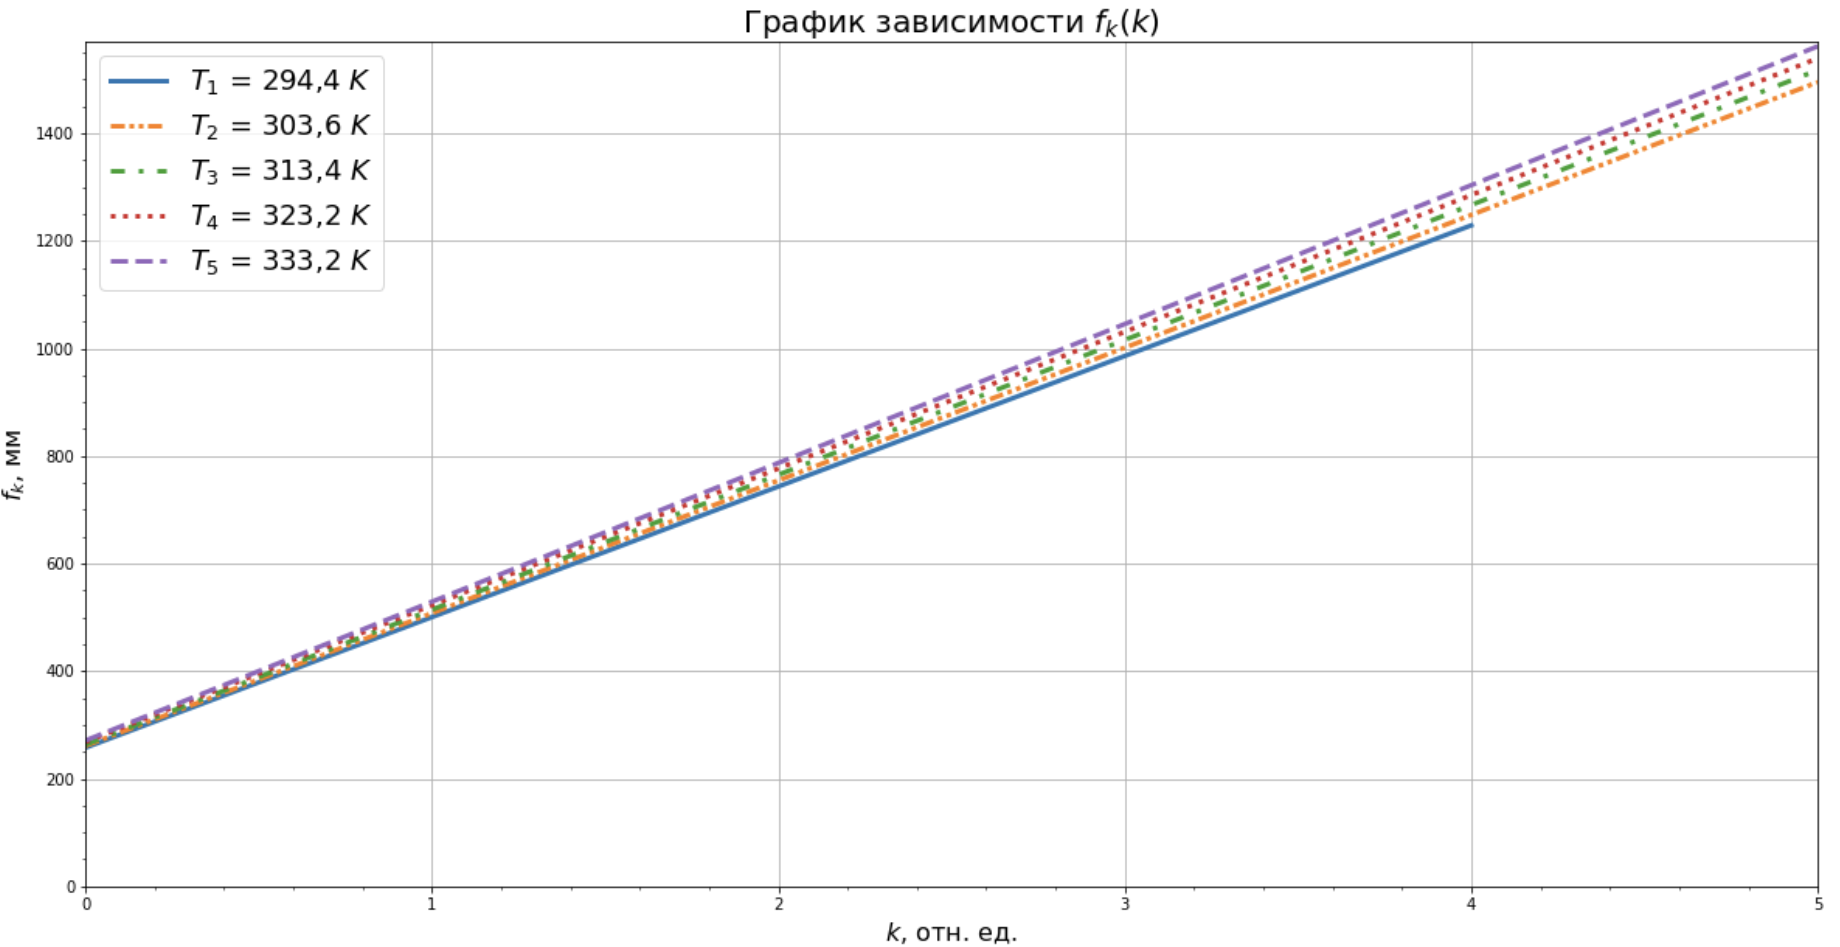
\includegraphics[scale=0.542]{graph2}
		\caption{Зависимость $ f_k $ от $ k $}
		\label{graph}
	\end{figure}

	Аппроксимируем полученные зависимости прямыми $ y=ax $ используя метод наименьших квадратов. Коэффициент $ a $ и погрешности его определения находим согласно формулам \eqref{mnk:a}, \eqref{mnk:sigma_a} и \eqref{mnk:full_sigma}. Результаты вычислений для каждой температуры заносим в таблицу \ref{tab:resConstL}.
	
	\begin{table}[H]
		\centering
		\begin{tabular}{|c|c|c|c|c|c|c|}
			\hline
			$ T $, К & $ a $, с$ ^{-1} $ & $ \sigma_a $, с$ ^{-1} $ & $ c $, м/с & $ \sigma_c $, м/с & $ \gamma $ & $ \sigma_\gamma $ \\ \hline
			294,4 & 242,8 & 1,3 & 339,9 & 1,8 & 1,369 & 0,007 \\ \hline
			303,6 & 246,9 & 0,9 & 345,7 & 1,3 & 1,373 & 0,005 \\ \hline
			313,4 & 250,8 & 1,0 & 351,1 & 1,4 & 1,372 & 0,005 \\ \hline
			323,2 & 254,3 & 0,9 & 356,0 & 1,3 & 1,368 & 0,005 \\ \hline
			333,2 & 258,2 & 0,8 & 361,5 & 01,2 & 1,368 & 0,005 \\ \hline
		\end{tabular}
		\caption{Результаты вычислений при различных температурах}
		\label{tab:resConstL}
	\end{table}
	
	Также, согласно формуле \eqref{5}, коэффициент наклона $ \displaystyle a = \frac{c}{2L}$. Тогда вычислим скорость звука $ c $ при фиксированной температуре и её погрешность, результаты вычислений занесём в таблицу \ref{tab:resConstL}.
	
	Кроме того, по формуле \eqref{gamma} вычислим $ \gamma $ при фиксированной температуре и погрешность этого вычисления. Результаты занесём в таблицу $ \ref{tab:resConstL} $. 
	
	Согласно полученным данным, можно утверждать, что $ \gamma $ остаётся постоянной в исследуемом диапазоне температур. Поэтому усредним результаты, полученные при различных значениях температуры и получим для воздуха:
	
	\[ \boxed{\gamma = 1,370 \pm 0,005}\quad (\varepsilon=0,4\%) \]
	
	\section{Обсуждение результатов и выводы}
	
	В ходе выполнения работы мы:
	
	\begin{itemize}
		\item измерили частоту колебаний и длину волны при резонансе звуковых колебаний в газе, заполняющем экспериментальную установку;
		\item определили разными методами показатель адиабаты с помощью уравнения состояния идеального газа.
	\end{itemize}
	
	В ходе работы показатель адиабаты для воздуха был измерен двумя разными способами. Сначала измерения проводились при фиксированной частоте звукового сигнала, а мы изменяли длину трубы. В ходе таких измерения было получено:
	
	\[ \boxed{\gamma_f = 1,412 \pm 0,008}\quad (\varepsilon=0,6\%) \]
	
	Затем измерения проводились на другой установке, на которой длина трубы оставалась постоянной на протяжении всего опыта, а резонанса мы добивались при помощи изменения частоты звукового сигнала. В ходе этих измерений также исследовалась зависимость коэффициента адиабаты $ \gamma $ от температуры газа. Было получено, что показатель адиабаты не зависит от температуры в диапазоне температур $ 20-60 $ $ ^\circ C $ и равняется:
	
	\[ \boxed{\gamma_L = 1,370 \pm 0,004}\quad (\varepsilon=0,6\%) \]
	
	Сравним полученные данные с табличными. Согласно справочнику, показатель адиабаты для воздуха при нормальных условиях равен \underline{$ \gamma = 1,4 $}. Таким образом, можно утверждать, что результат измерения $ \gamma $ на первой установке в пределах погрешности совпадает с табличными данными. Результаты измерения на второй установке незначительно отличаются от табличных. Это может быть связано с большой неточностью определения резонансных частот на второй установке. Чтобы этого избежать, необходимо использовать генератор частоты с возможностью более точной настройки для возможности четкого отслеживания резонансов.
	
	Также в ходе работы был измерен показатель адиабаты для углекислого газа. Измерения проводились на первой установке. В итоге мы получили \[ \boxed{\gamma_{CO_2} = 1,271 \pm 0,016}\quad (\varepsilon=1,4\%) \]
	
	Сравним эти данные с табличными. Согласно справочнику, показатель адиабаты для углекислого газа при нормальных условиях \underline{$ \gamma = 1,3 $}. Таким образом, полученные данные незначительно отличаются от табличных. Это может быть связано с тем, что при измерениях в трубе находился углекислый газ с примесями (в основном, азот и кислород), которые могли исказить результаты измерений. Для повышения точности, эксперимент стоит проводить в атмосфере углекислого газа, чтобы исключить попадание различных примесей в трубу.
	
	
	
	
	
	
\end{document}